\section{Single Shooting}
The optimization problem can be formulated as an nlp with the system dynamics as constraints. To avoid persistent strict policies, the cost function decreases quadratically with $u_k$. This can be viewed as a penalty modelling the negative impacts of lockdown.

\begin{mini*}|s|
{w}{\sum_{k=1}^NI_k^2 -W_u u_{k-1}^2}
{}{}
\addConstraint{x_f = f(x_0, [u_0, \dots, u_{N-1}])}
\addConstraint{u_{max} \geq u_k \geq u_{min}}{}
\end{mini*}
Where $f(.)$ is the trajectory from initial to end state. The intermediate states of the system is not visible to the solver. $f(.)$ can be implemented as an iterative RK4-scheme:

\begin{algorithm}[H]
\SetAlgoLined
\KwData{$x_k = x_0, u = [u_0, \dots, u_{N-1}], h, N$}
 \For{$i$ = 0 : $N-1$}{
    $x_k, Q_k = RK4(@SIR,@Cost, x_k, u_k, h)$\\
    $J += Q_k$\\
    Set boundaries and initial value for $u_k$
 }
 \KwRet{$x_k, J$, \text{boundaries and initial values}}
 \caption{Single-shooting problem construction and integration}
 \label{alg:SingleShooting_Integraion}
\end{algorithm}

The resulting variables, values and boundaries can be directly inserted into the CasADI-interface if derived symbolically, or directly intefaced with a solver when derived numerically.
\iffalse
\subsection{Optimal Control using IPOPT interfaced by CasADI}
The problem is formulated using CasADI in Python, where a single step of algorithm \ref{alg:SingleShooting_Integraion} is formulated with MX-symbolics and transformed to a CasADI-function. $u = [u_0, \dots, u_{N-1}]$ is initialized as a MX-variable and elementwise inserted into the function for each for-loop step in algorithm \ref{alg:SingleShooting_Integraion}. Boundaries are added to $u$, resulting in lists which can be inserted into the CasADI's solver framework.

Optimal control is solved using default parameters and initial conditions from \ref{ch:Problem_Parameters}.

\fi



\subsection{Primal-Dual Interior Point Formulation}
The inequalities can be replaced using the log-barrier method:

\begin{mini*}|s|
{w_\tau}{\Phi(w_\tau) - \tau \sum_{k=0}^{N-1}(\log(u_k-u_{min}) + \log(u_{max}-u_k))}
{}{}
\addConstraint{x_f = f(x_0, [u_0, \dots, u_{N-1}])}
\end{mini*}
\begin{align}
    h(w_\tau) &= \begin{bmatrix} u_0-u_{min} \\ u_{max}-u_0 \\ \vdots \\
u_{max}-u_{N-1}
    \end{bmatrix}& 
 \nu&= -\tau \begin{bmatrix}
h_0^{-1}\\ \vdots \\ h_{2(N-1)}^{-1} \end{bmatrix}
\end{align}
Which gives the Primal-Dual KKT-conditions:
\begin{align}
    \nabla \Phi(w) + \nabla h(w)\nu + \nabla f(x_0, [u_0, \dots, u_{N-1}])\lambda &= 0\nonumber \\
    g(w) = x_f-f(x_0, [u_0, \dots, u_{N-1}]) &= 0\\\nonumber
    \nu_ih_i(w) + \tau &= 0 \\\nonumber
    h(w) < 0, \nu &> 0
\end{align}
The complementarity slackness in the Primal-Dual method approximates the constraints for the original formulation, and will converge to $\mu$ for small $\tau$. The current formulation requires $h(w) < 0$, which can be relaxed with slack variable $s$. Furthermore, the problem can be expressed in terms of true KKT conditions by setting $\nu = \mu$, which upper bounds the optimum error $\mu^*-\nu^*$ linearly with $\tau$. This results in equation \ref{eq:KKT_approx_IPOPT}, where the equalities can be used for Newton-Rhapson steps.

\begin{align}
        \nabla \Phi(w) + \nabla h(w)\nu + &\nabla f(x_0, [u_0, \dots, u_{N-1}])\lambda = 0 \nonumber \\ 
        g(w) &= 0\nonumber \label{eq:KKT_approx_IPOPT}\\
    h_i(w) + s &= 0\\\nonumber
    \mu_is_i-\tau &= 0\\\nonumber
    s > 0, \mu &> 0
\end{align}

\subsection{CasADI using the IPOPT-solver}
\subsubsection{Implementation}
Single-shooting is implemented in CasADI using $X_0 \in \mathbb{R}^3, U \in \mathbb{R}^{N}$ as MX-variables. The ODE is integrated $M$ times for each control interval, resulting in a total of $N\times M$ integration steps. Inequality constraints are passed as variable bounds, while equality constraints are passed as regular constraints to the solver.

\begin{algorithm}[H]
\SetAlgoLined
\KwData{$x_k = x_0, U = MX \in \mathbb{R}^{N}, J=0, h, N$}
Construct integrator $f(ODE, x, u, h)$ with CasADI-symbolics\\
 \For{$i$ = 0 : $N-1$}{
    $x_k, Q_k$ = $f([@SIR, @Cost\_ODE], x_k, U[i], h)$\\
    $J+= Q_k$\\
 }
 solver = nlpsol('solver', 'ipopt', $\{$J, $U\}$)\\
 sol = solver($x_0$, $U_{min}$, $U_{max}$)
 \caption{Single-shooting with IPOPT}
 \label{alg:SingleShooting_Integration_IPOPT}
\end{algorithm}
\subsubsection{Results}
Simulating with parameters defined in section \ref{ch:Problem_Parameters} yields the following results:

\begin{figure}[H]
    \centering
    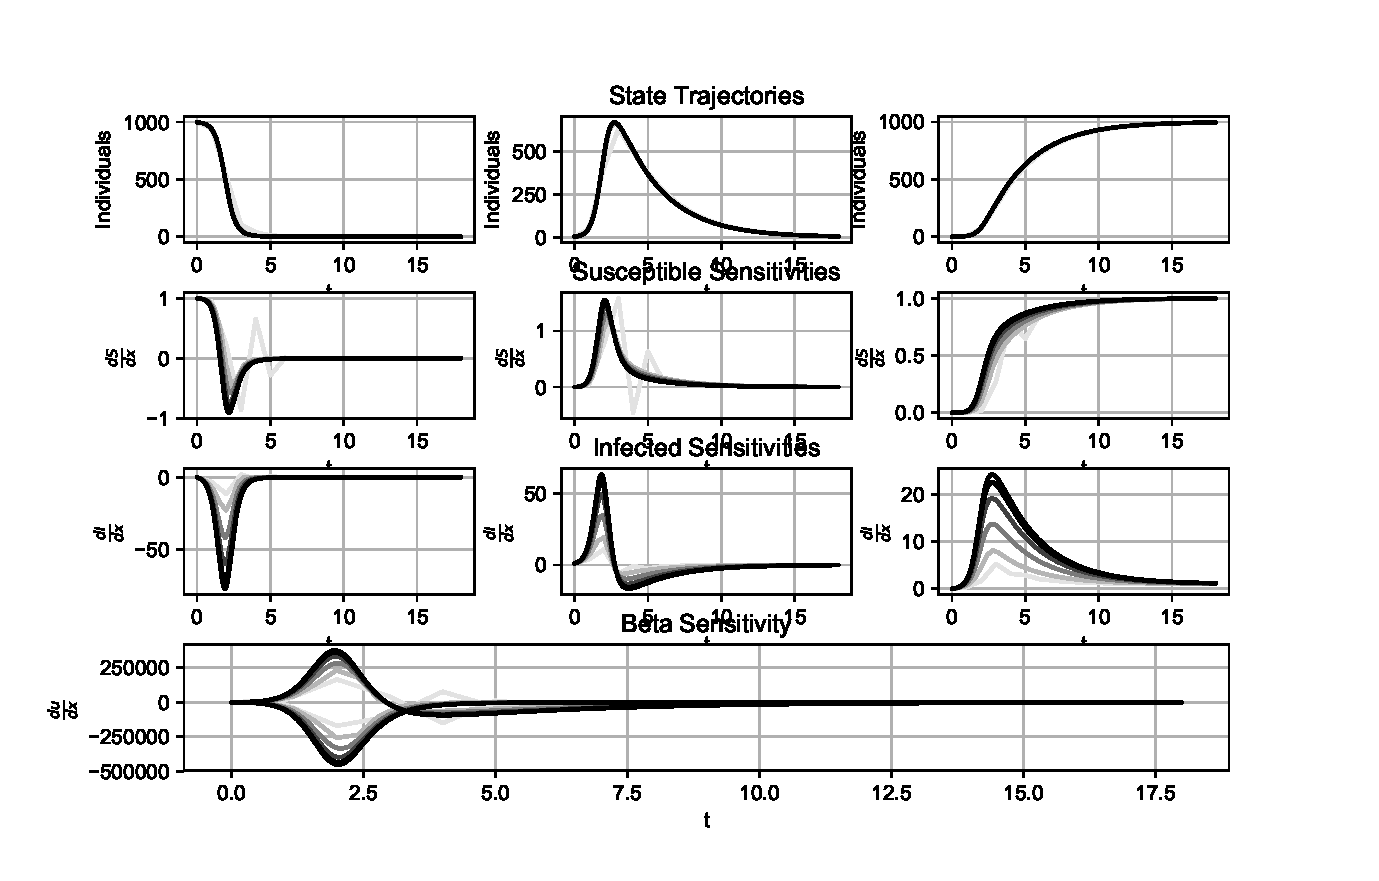
\includegraphics{pythonProject/Figures/Variational_Sensitivities.eps}
    \caption{Caption}
    \label{fig:Trajectories for the Single}
\end{figure}

\subsection{CasADI-Implementation using }